\documentclass{X:/Documents/Coding/Latex/myassignment}
\title{Topic C Project}

\begin{document}

\maketitle

The paper, \textit{Analytical solution of amperometric enzymatic reactions based on
Homotopy perturbation method} by Shanmugarajana et al uses a homotopy perturbation method to obtain a solution to a set of non-linear diffusion equations giving a general mathematical description the reaction of electrochemical polymerisation.

Using homotopy they get the system

\begin{align*}
	(1-p)\left(\frac{d^2s}{dx^2} - \kappa s\right) + p \left(\frac{d^2s}{dx^2} + \alpha s \frac{d^2s}{dx^2} - \kappa s\right) = 0\\
	(1-p)\left(\frac{d^2b}{dx^2} - \eta s\right) + p \left(\frac{d^2b}{dx^2} + \alpha s \frac{d^2b}{dx^2} - \eta s\right) = 0
\end{align*}
With boundary conditions 
\[x=0 ; \quad \odd sx = 0; \quad b=0\]

\[x=l ; \quad s = Ks_{\infty}; \quad b=0\]
Where $l$ is the distance between the electrode and the solution.

Variables and parameters
\begin{itemize}
	\item $s$ is the substrate concentration
	\item $b$ is the concentration of the mediator
	\item $x$ is the position
	\item $Ks_{\infty}$ is the surface concentration of substrate
	\item $l$ is the film thickness
	\item $\alpha,\kappa,\eta$ are constant parameters
\end{itemize}

I will redo the \textit{leading order solutions} using perturbation methods. Skipping to the point after the homotopy is applied, the system is
Which simplifies to
\begin{align*}
	\frac{d^2s}{dx^2} - \kappa s + p \alpha s \frac{d^2s}{dx^2} = 0\\
	\frac{d^2b}{dx^2} + \eta s + p \alpha s \frac{d^2b}{dx^2} = 0
\end{align*}

\[
\alpha := \frac{k_{cat} + ka}{K_Mka},\quad \kappa := \frac{k_{cat} e_{\Sigma}}{D_sK_M} \quad and \quad \eta := \frac{k_{cat}e_{\Sigma}}{D_BK_M}
\]

Take the perturbation series
\[s = \sum_{n=0}^\infty p^n s_n = s_0 + ps_1 + \bigo(p^2)\]
And
\[b = \sum_{n=0}^\infty p^n b_n = b_0 + pb_1 + \bigo(p^2)\]

Sub into the system to order $\bigo(p)$
First equation:
\begin{align*}
	&\frac{d^2}{dx^2}(s_0 + ps_1 + \bigo(p^2)) - \kappa (s_0 + ps_1 + \bigo(p^2)) + p \alpha (s_0 + ps_1 + \bigo(p^2))\frac{d^2}{dx^2}(s_0 + ps_1 + \bigo(p^2)) = 0\\
	&\bigo(p^0) : \quad \frac{d^2s_0}{dx^2} - \kappa s_0 = 0\\
	&\bigo(p) : \quad \frac{d^2s_1}{dx^2} - \kappa s_1 +  \alpha s_0 \frac{d^2s_0}{dx^2} = 0\\
\end{align*}
Second equation:
\begin{align*}
	&\frac{d^2}{dx^2}(b_0 + pb_1 + \bigo(p^2)) + \eta (s_0 + ps_1 + \bigo(p^2)) + p \alpha (s_0 + ps_1 + \bigo(p^2)) \frac{d^2}{dx^2}(b_0 + pb_1 + \bigo(p^2)) = 0\\
	&\bigo(p^0) : \quad	\frac{d^2b_0}{dx^2} + \eta s_0  = 0\\
	&\bigo(p) : \quad \frac{d^2b_1}{dx^2}+ \eta s_1 + \alpha s_0 \frac{d^2b_0}{dx^2} =0
\end{align*}


Solve for $s_0$:
\begin{align*}
	\frac{d^2s_0}{dx^2} - \kappa s_0 = 0\\
	\implies s_0 = c_1\cosh(\sqrt{\kappa} x) + c_2 \sinh(\sqrt{\kappa}x)
\end{align*}
Applying boundary conditions:
To leading order the BCs are identical: $\odd{s_0}x\pipe_{x=0} = 0$ and $s_0|_{x=l} = Ks_{\infty}$
\begin{align*}
	\odd{s_0}{x} =  c_2\sqrt{\kappa}\cosh(\sqrt{\kappa} x) + c_1 \sqrt{\kappa}\sinh(\sqrt{\kappa}x)\\
	\odd{s_0}{x}\pipe_{x=0} =  c_2\sqrt{\kappa} = 0\\
	\implies c_2 =0 
\end{align*}
And 
\begin{align*}
	s_0\pipe_{x=l} = c_1\cosh(\sqrt{\kappa} l) = Ks_{\infty}\\
	\implies c_1 = \frac{Ks_{\infty}}{\cosh(\sqrt{\kappa} l)}
\end{align*}
So 
\[\boxed{s_0 = \frac{Ks_{\infty}\cosh(\sqrt{\kappa} x)}{\cosh(\sqrt{\kappa} l)}}\]

$b_0$:
\begin{align*}
	\frac{d^2b_0}{dx^2} + \eta s_0  = 0\\
	\frac{d^2b_0}{dx^2} +\frac{\eta Ks_{\infty}\cosh(\sqrt{\kappa} x)}{\cosh(\sqrt{\kappa} l)} =0\\
	b_0 = Ax + B - \frac{\eta Ks_{\infty}\cosh(\sqrt{\kappa} x)}{\kappa\cosh(\sqrt{\kappa} l)}\\
\end{align*}

\begin{align*}
	b_0\pipe_{x=0} = B - \frac{\eta Ks_{\infty}\cosh(0)}{\kappa\cosh(\sqrt{\kappa} l)} = 0\\
	\implies B =\frac{\eta Ks_{\infty}}{\kappa\cosh(\sqrt{\kappa} l)}
\end{align*}

\begin{align*}
	b_0\pipe_{x=l} = Al + \frac{\eta Ks_{\infty}}{\kappa\cosh(\sqrt{\kappa} l)} - \frac{\eta Ks_{\infty}\cosh(\sqrt{\kappa} l)}{\kappa\cosh(\sqrt{\kappa} l)} = 0\\
	A = \frac{\eta Ks_{\infty}}{l\kappa\cosh(\sqrt{\kappa} l)} \left(\cosh(\sqrt{\kappa} l) -1\right) \\
\end{align*}


Hence
\begin{align*}
	b_0 &= \frac{x\eta Ks_{\infty}}{l\kappa\cosh(\sqrt{\kappa} l)} \left(\cosh(\sqrt{\kappa} l) -1\right)+ \frac{\eta Ks_{\infty}}{\kappa\cosh(\sqrt{\kappa} l)} - \frac{\eta K s_{\infty}\cosh(\sqrt{\kappa} x)}{\kappa \cosh(\sqrt{k}l)}\\
	b_0 &=\frac{\eta K s_{\infty}}{\kappa\cosh(\sqrt{k}l)} \left(\frac xl(\cosh(\sqrt{\kappa l}) - 1) + 1 - \cosh(\sqrt{k}x)\right)
\end{align*}

Which is the same as derived in the paper.









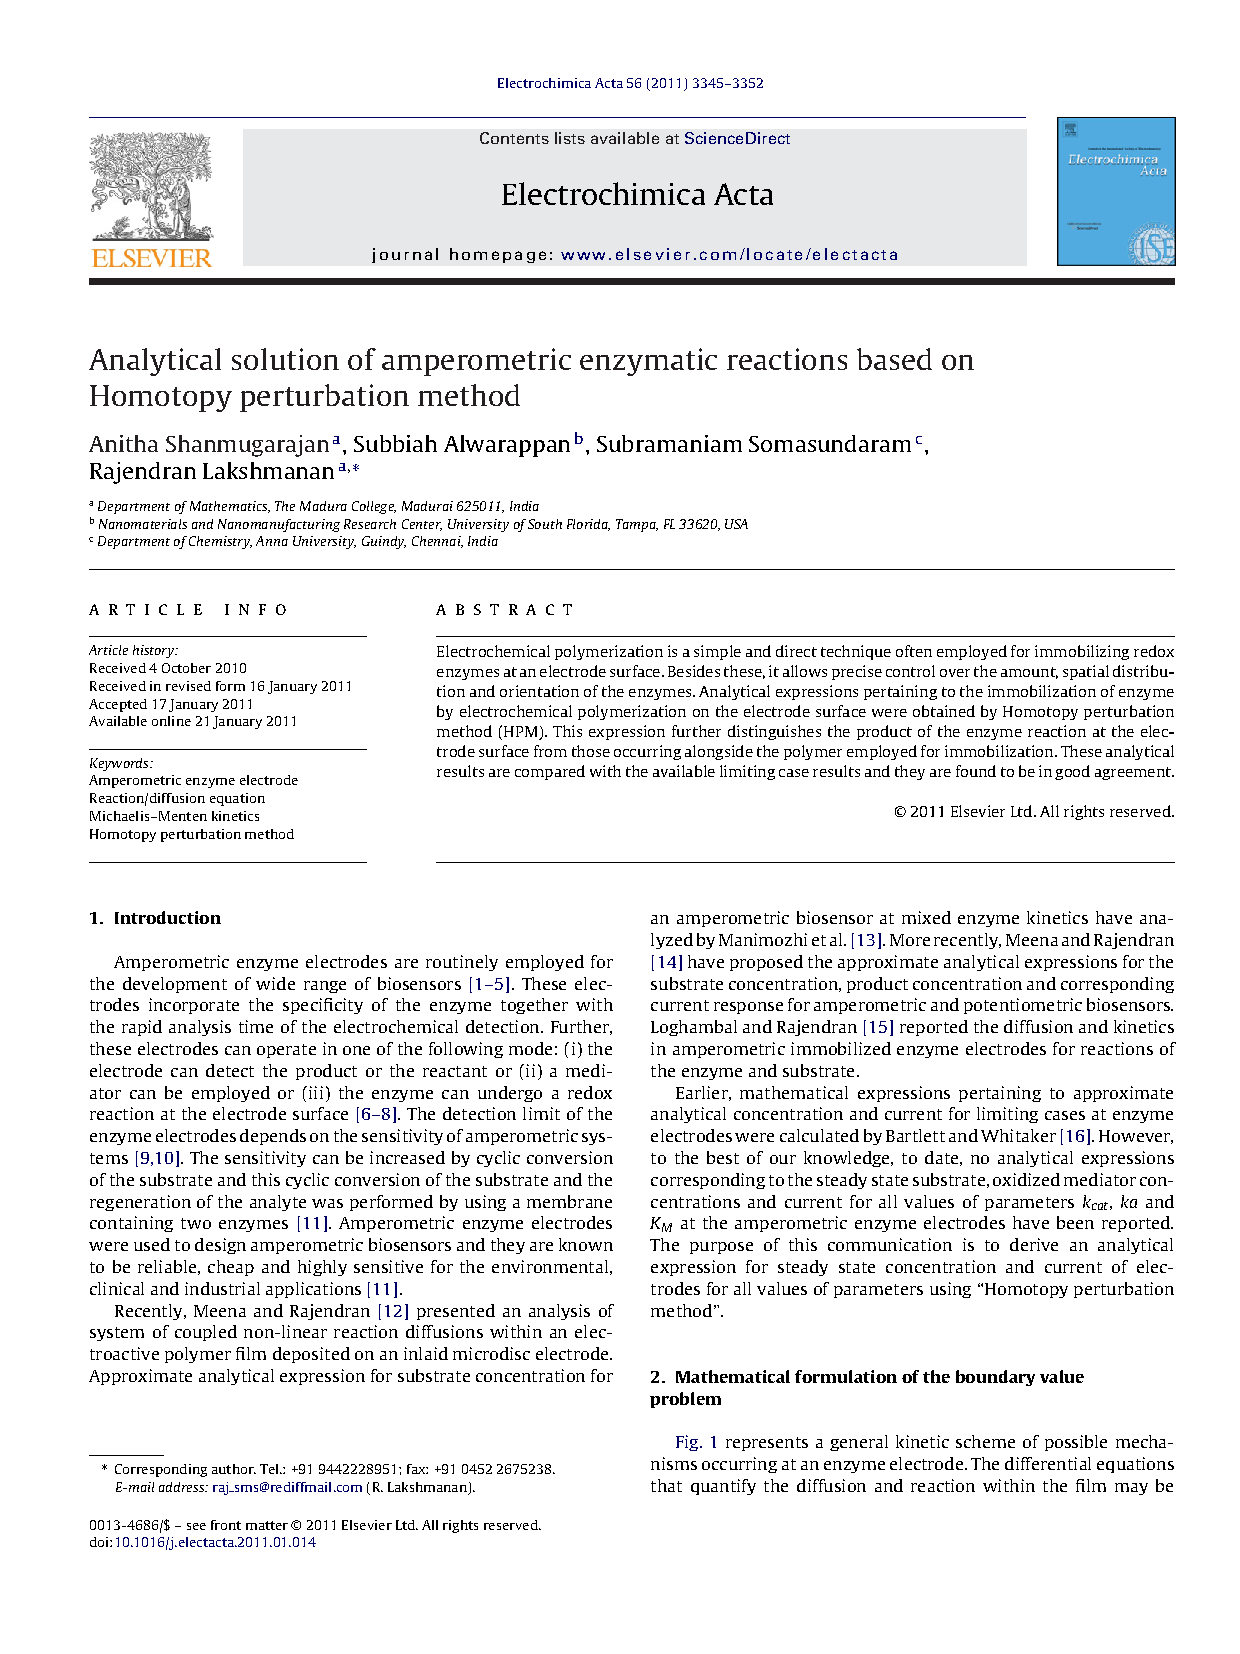
\includepdf[pages=1-]{paper.pdf}
\end{document}